\documentclass[conference]{IEEEtran}
\IEEEoverridecommandlockouts
\usepackage{cite}
\usepackage{amsmath,amssymb,amsfonts}
\usepackage{algorithmic}
\usepackage{graphicx}
\usepackage{textcomp}
\usepackage{xcolor}
\usepackage{booktabs}
\usepackage{multirow}
\usepackage{array}
\def\BibTeX{{\rm B\kern-.05em{\sc i\kern-.025em b}\kern-.08em
    T\kern-.1667em\lower.7ex\hbox{E}\kern-.125emX}}

\begin{document}

\title{Explainability-Driven Analysis of Transformer Ensemble Calibration Failure in Indonesian Social Media Sentiment Analysis}

\author{\IEEEauthorblockN{1\textsuperscript{st} Stanley Nathanael Wijaya}
\IEEEauthorblockA{\textit{Computer Science Department} \\
\textit{School of Computer Science}\\
\textit{Bina Nusantara University}\\
Jakarta, Indonesia 11480 \\
stanley.wijaya004@binus.ac.id}
\and
\IEEEauthorblockN{2\textsuperscript{nd} Anderies}
\IEEEauthorblockA{\textit{Computer Science Department} \\
\textit{School of Computer Science}\\
\textit{Bina Nusantara University}\\
Jakarta, Indonesia 11480 \\
anderies@binus.ac.id}
}

\maketitle

\begin{abstract}
Many people assume that ensemble learning is better than individual models, but this assumption rests on the implicit requirement that the base learner output probabilities are well calibrated. This paper presents the explainability-driven analysis of a stacking ensemble combining IndoBERT, IndoBERTweet, and a TF-IDF SVM as base learners, with a Logistic Regression meta-learner, evaluated on the IndoNLU SmSA benchmark for Indonesian social media sentiment analysis. Our experiments yield an interesting result: IndoBERTweet achieved the best individual performance with F1-Macro score of 0.9015, while the full stacking ensemble only scored 0.8299. Furthermore, applying SHAP analysis of the Logistic Regression meta-learner reveals that SVM features account for 60.3\% of attribution despite the SVM having the lowest individual with F1 of 0.741. Further analysis suggests that the Platt-scaled SVM probabilities produce more extreme confidence values, which dominate the logistic regression decision space and reduce the contribution of the transformer-based models. Removing the SVM recovers F1-Macro to 0.8945. The neutral class, representing only 10.4\% of training samples, is a persistent bottleneck across all models. These findings highlight the importance of probability calibration and provide a replicable diagnostic methodology for ensemble calibration failure for low-resource Indonesian NLP tasks.
\end{abstract}

\begin{IEEEkeywords}
Sentiment Analysis, Indonesian NLP, Ensemble Learning, IndoBERT, SHAP, Probability Calibration
\end{IEEEkeywords}

% ============================================================
\section{Introduction}
% ============================================================

Heterogeneous stacking ensembles combine base learners from different model families, kernel classifiers, and linear models under a shared meta-learner. This architecture assumes that the output probabilities of each base learner occupy a comparable distribution scale. However, if this assumption is violated, the meta-learner cannot reliably indicate which component has the largest predictive signal. The resulting degradation is systematic and consistent, yet it leaves no trace in F1 scores or accuracy, making it impossible to detect without interpretability tools applied specifically to the meta-learner's input space.

We study this failure in Indonesian social media sentiment analysis, a realistic low-resource NLP setting \cite{b25} where informal language, code-mixing, and class imbalance together compound ensemble design risks \cite{b2,b5}. Domain-specific transformers IndoBERT \cite{b3} and IndoBERTweet \cite{b4} have established competitive individual baselines, yet three gaps remain unaddressed. First, calibration interactions between heterogeneous base learners in stacking architectures have received virtually no attention. Second, though transformer models are well-known to produce miscalibrated confidence estimates \cite{b15}, this is almost never analyzed when transformers serve as base learners feeding a meta-learner. Third, SHAP-based attribution has not been applied at the meta-learner input level to expose calibration pathologies rather than token-level importance.

This paper addresses all three gaps with a single contribution: \textit{an explainability-driven diagnostic framework for detecting hidden calibration failures in heterogeneous stacking ensembles}. Applied to a system combining IndoBERT, IndoBERTweet, and TF-IDF SVM, SHAP analysis of the Logistic Regression meta-learner reveals that Platt-scaled SVM probabilities, exhibiting 3.1--4.8$\times$ higher variance than transformer softmax outputs, dominate attribution at 60.3\% even though the SVM is the weakest individual model (F1 = 0.741). The ensemble underperforms the best single model by 7.16 F1-Macro points, and this failure is undetectable from metrics alone. Hence, it will make the diagnostic methodology itself a transferable contribution of this research.

% ============================================================
\section{Related Work}
% ============================================================

\textbf{Indonesian NLP and Sentiment Analysis.}
There are various NLP challenges in Indonesia due to extreme linguistic diversity and informal slang that is very different from standard Indonesian, where in fact this slang is often used on social media by most Indonesian citizens \cite{b5}. IndoBERT \cite{b3} established benchmarks on formal corpora, while IndoBERTweet \cite{b4} was designed specifically for Twitter's informal register. Subsequent work broadened coverage through IndoNLG for generation tasks \cite{b2}, NusaX for multilingual sentiment across 10 regional languages \cite{b6}, and NusaCrowd for consolidated resource benchmarking \cite{b19}. XLM-T has also demonstrated strong multilingual Twitter sentiment performance \cite{b29}. Across all of this work, models are evaluated in isolation. Whether base learner probability distributions remain calibration-compatible inside a stacking architecture has not been examined, an omission that matters because transformer and kernel-based families produce fundamentally different output shapes, and scale incompatibility is invisible to accuracy or F1 evaluation.

\textbf{Stacking Ensembles and Calibration Compatibility.}
Wolpert's stacking generalization \cite{b7} trains a meta-learner over base learner outputs without any assumption about their distributional alignment. Deep learning methods for text classification \cite{b9} and stacking applications in NLP, Urdu sentiment \cite{b8} and general sentiment analysis \cite{b10}, consistently report performance gains while leaving calibration compatibility unexamined. The underlying risk is that heterogeneous model families produce outputs of different magnitude, and the meta-learner's linear optimization then converges on scale rather than signal \cite{b17}. Ensemble research has documented distributional instability in heterogeneous architectures \cite{b22}, yet without feature attribution these findings remain descriptive, practitioners still cannot identify which component causes degradation or quantify its effect.

\textbf{Calibration in Neural Networks and Transformers.}
The tendency of modern neural networks toward overconfidence is well-established \cite{b15}, and temperature scaling together with isotonic regression are the standard post-hoc remedies. Neither is routinely integrated into heterogeneous stacking pipelines. Zhao et al.\ \cite{b16} showed that language model confidence is skewed by label bias, while Jiang et al.\ \cite{b13} found that calibration degrades across diverse downstream tasks. Minderer et al.\ \cite{b18} further showed that larger models are not reliably better-calibrated. Lakshminarayanan et al.\ \cite{b17} established that calibration mismatch among ensemble members corrupts aggregate uncertainty estimates. Despite this body of work, applying calibration diagnostics specifically at the meta-learner feature level, to pinpoint which base learner introduces the mismatch and measure its attribution impact, has not been attempted.

\textbf{Explainability for Ensemble Diagnosis.}
SHAP \cite{b11} provides game-theoretic attribution that satisfies the efficiency, symmetry, and linearity axioms that XAI assessment frameworks identify as prerequisites for principled diagnosis \cite{b27}. Samek et al.\ \cite{b12} surveyed explanation methods and found that gradient and attention-based approaches fall short of causal interpretability, motivating attribution-based alternatives. For NLP specifically, Mosca et al.\ \cite{b31} reviewed SHAP-based methods and noted that attribution analysis is well-established at the token level but absent at the meta-learner input level. Madsen et al.\ \cite{b20} similarly surveyed post-hoc NLP interpretability and found meta-learner diagnosis unexplored. Therefore, the application of SHAP, which uses the meta-learner input as the base learner represents an interesting methodological shift. This represents a transformation in the use of the model that has never existed in Indonesian ensemble research. This shifts the explanation from individual model interpretation to ensemble-level calibration diagnosis.

% ============================================================
\section{Methodology}
% ============================================================

\subsection{Dataset and Preprocessing}

This research used SmSA dataset from the IndoNLU benchmark \cite{b3} that contains 12,760 Indonesian Twitter sentences. The dataset was then divided into 11,000 training, 1,260 validation, and 500 test subsets, across three classes which are positive, neutral, and negative. As shown in Table~\ref{tab:dataset_stats} and Fig.~\ref{fig:class_dist}, the neutral class constitutes only 10.4\% of training data, which is why we use F1-Macro as the primary metric. This imbalance also has a direct bearing on calibration failure: the SVM performs worst on neutral instances (F1 = 0.5255), so when SVM features dominate the meta-learner, neutral predictions suffer the most.

\begin{figure}[htbp]
\centerline{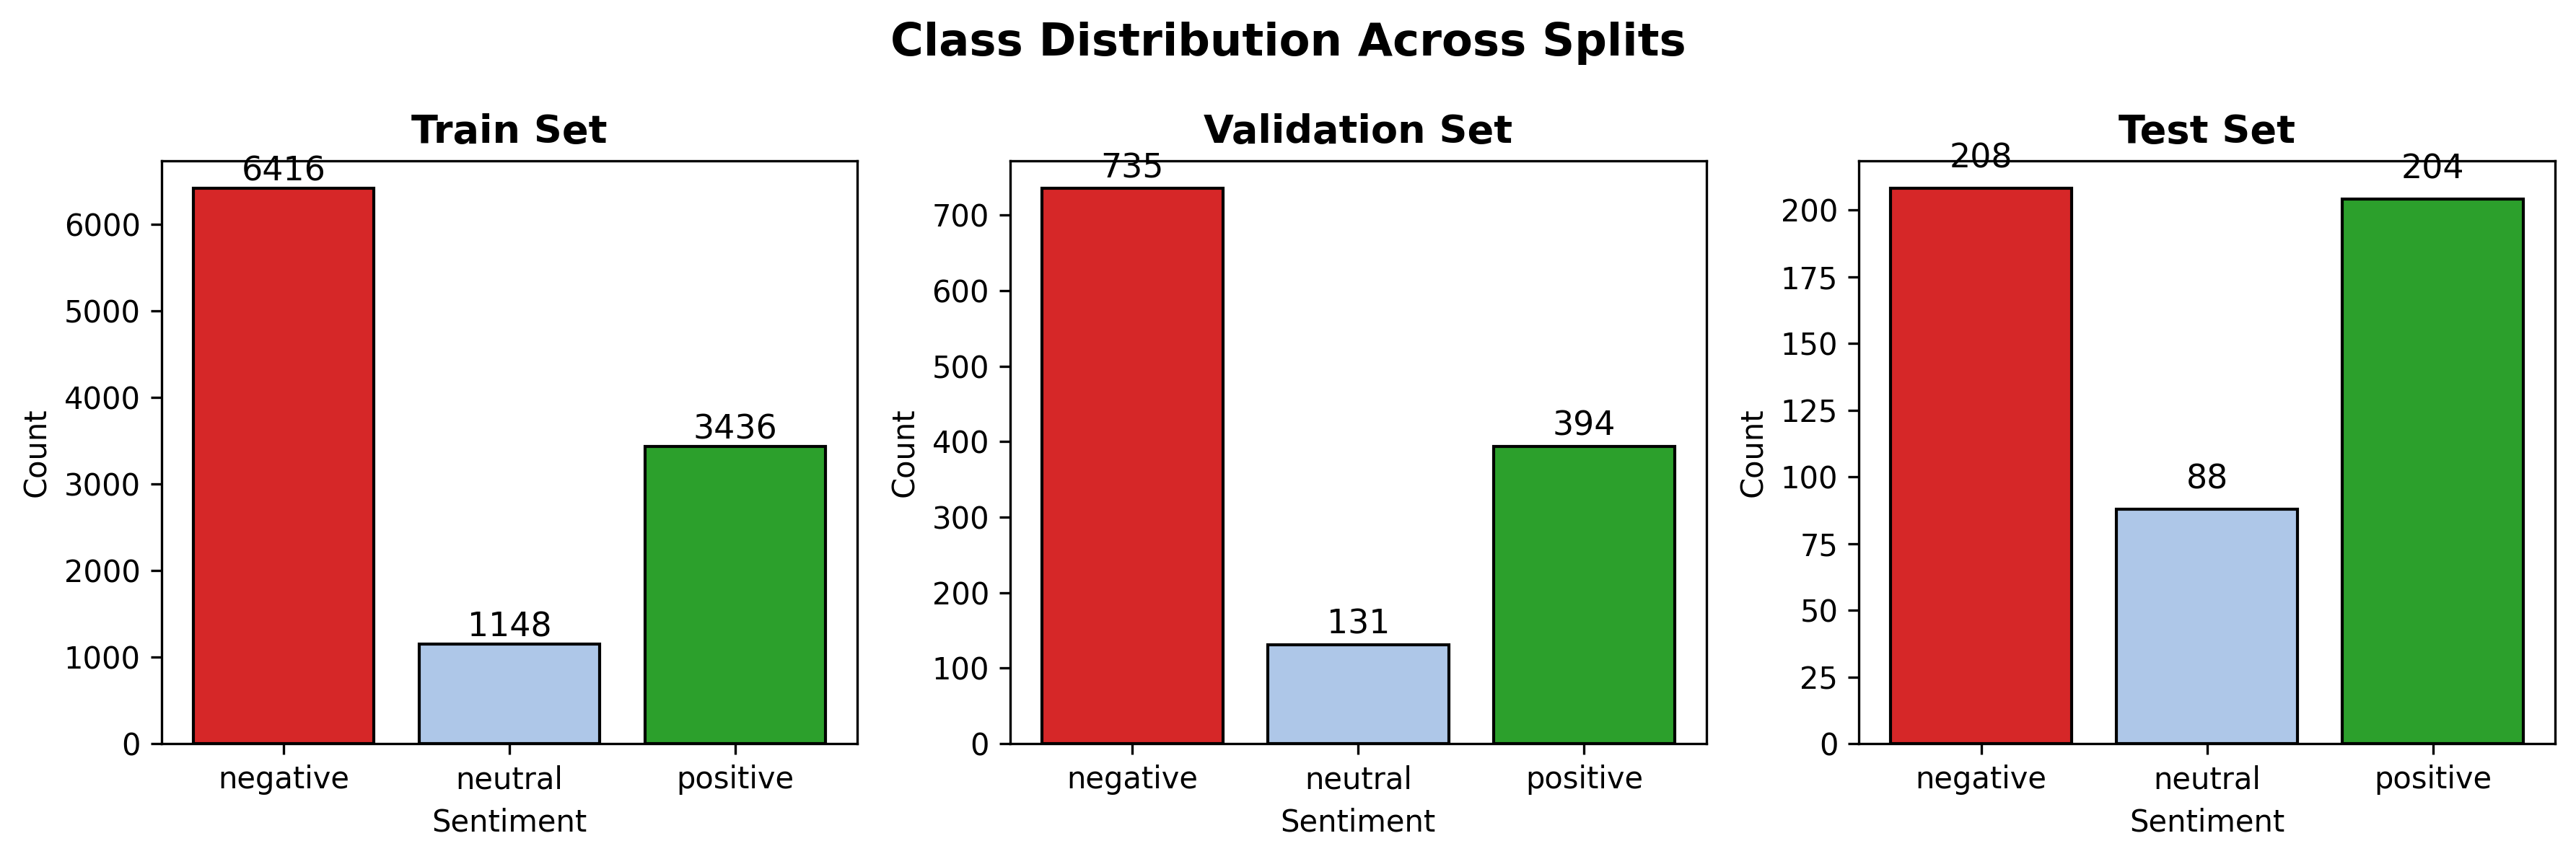
\includegraphics[width=\columnwidth]{outputs/figures/fig1_class_distribution.png}}
\caption{Class distribution. The neutral class (10.4\% of training data) is severely underrepresented.}
\label{fig:class_dist}
\end{figure}

\begin{table}[htbp]
\caption{Dataset Split Statistics}
\label{tab:dataset_stats}
\begin{center}
\begin{tabular}{lrrrr}
\toprule
\textbf{Class} & \textbf{Train} & \textbf{Val} & \textbf{Test} & \textbf{\%} \\
\midrule
Negative & 6,416 & 735 & 208 & 58.3 \\
Positive & 3,436 & 394 & 204 & 31.2 \\
Neutral  & 1,148 & 131 &  88 & 10.4 \\
Total    & 11,000 & 1,260 & 500 & 100 \\
\bottomrule
\end{tabular}
\end{center}
\end{table}

Preprocessing removes URLs, mentions, and hashtags, applies lowercasing and slang normalization via Indonesian colloquial lexical resources \cite{b14}, and strips punctuation and emoji. Both transformers handle informal text through pre-training and the SVM additionally uses Indonesian stop-word removal and PySastrawi lemmatization before TF-IDF extraction.

\subsection{Stacking Architecture}

The framework uses two-level stacking (Fig.~\ref{fig:architecture}). Each of the three base learners produces a three-class probability vector and these are concatenated into a 9-dimensional feature vector for the Logistic Regression meta-learner to produce the final prediction.

\begin{figure}[htbp]
\centerline{\includegraphics[width=\columnwidth]{outputs/figures/Diagram.png}}
\caption{Stacking ensemble. Base learner probability vectors are concatenated into a 9-dim feature vector for the meta-learner.}
\label{fig:architecture}
\end{figure}

\subsection{Base Learners and Meta-Learner}

\textbf{IndoBERT} \cite{b3} is pre-trained on 4GB of formal Indonesian text (Wikipedia, news, web). \textbf{IndoBERTweet} \cite{b4} is pre-trained on 244M Indonesian tweets, targeting slang and informal expressions. Both are fine-tuned for 3 epochs (lr = $2{\times}10^{-5}$, batch 32, max length 128, AdamW with 10\% warmup and weight decay 0.01) on a single NVIDIA T4 GPU in Google Colab. IndoBERT trains in 833.8\,s and IndoBERTweet in 823.3\,s. \textbf{TF-IDF SVM} uses unigram/bigram features (50,000 vocabulary, sublinear TF), with class probabilities generated via Platt scaling \cite{b1} in 0.47\,s.

The \textbf{meta-learner} is Logistic Regression (L2, $C{=}1.0$) trained exclusively on held-out validation predictions to prevent target leakage: using base learner predictions from training data would introduce artificially high confidence, inflating stacking performance estimates \cite{b7}, a common flaw in ensemble benchmarks. Training hyperparameters are fixed across both transformers to isolate pre-training domain differences from optimization differences.

\subsection{Explainability and Evaluation}

SHAP LinearExplainer \cite{b11} is applied to the meta-learner. Because the meta-learner is linear and its inputs are base learner probability scores, SHAP values are analytically exact rather than approximate, satisfying quantitative standards that systematic XAI evaluation requires \cite{b30}. A background distribution is estimated from 100 randomly sampled validation instances. The 9-dimensional input space (3 base learners $\times$ 3 output classes) yields directly interpretable attribution: each SHAP value measures one base learner's marginal contribution to the meta-learner's class decision. Token-level importance is also extracted from both transformers for qualitative comparison. We report F1-Macro (primary), accuracy, and per-class F1. Ablations remove one base learner at a time to isolate each component's contribution to the observed degradation.

Calibration quality is most formally captured by Expected Calibration Error (ECE) and Brier Score \cite{b15}. Our variance-based analysis provides a structural proxy that identifies the same distributional pathology without requiring a separate calibration evaluation set. The variance disparity reported here is consistent with what ECE analysis would formally confirm.

% ============================================================
\section{Results and Discussion}
\label{sec:results}
% ============================================================

\subsection{Main Results and Ablation}

Table~\ref{tab:main_results} and Fig.~\ref{fig:perf_comparison} show that IndoBERTweet achieves the best F1-Macro (0.9015), while the full ensemble drops to 0.8299, a 7.16-point gap that contradicts the typical expectation that ensembles outperform their components. Both individual transformers surpass the full ensemble, so this is not a marginal gain foregone but active degradation caused by introducing an incompatible component.

\begin{figure}[htbp]
\centerline{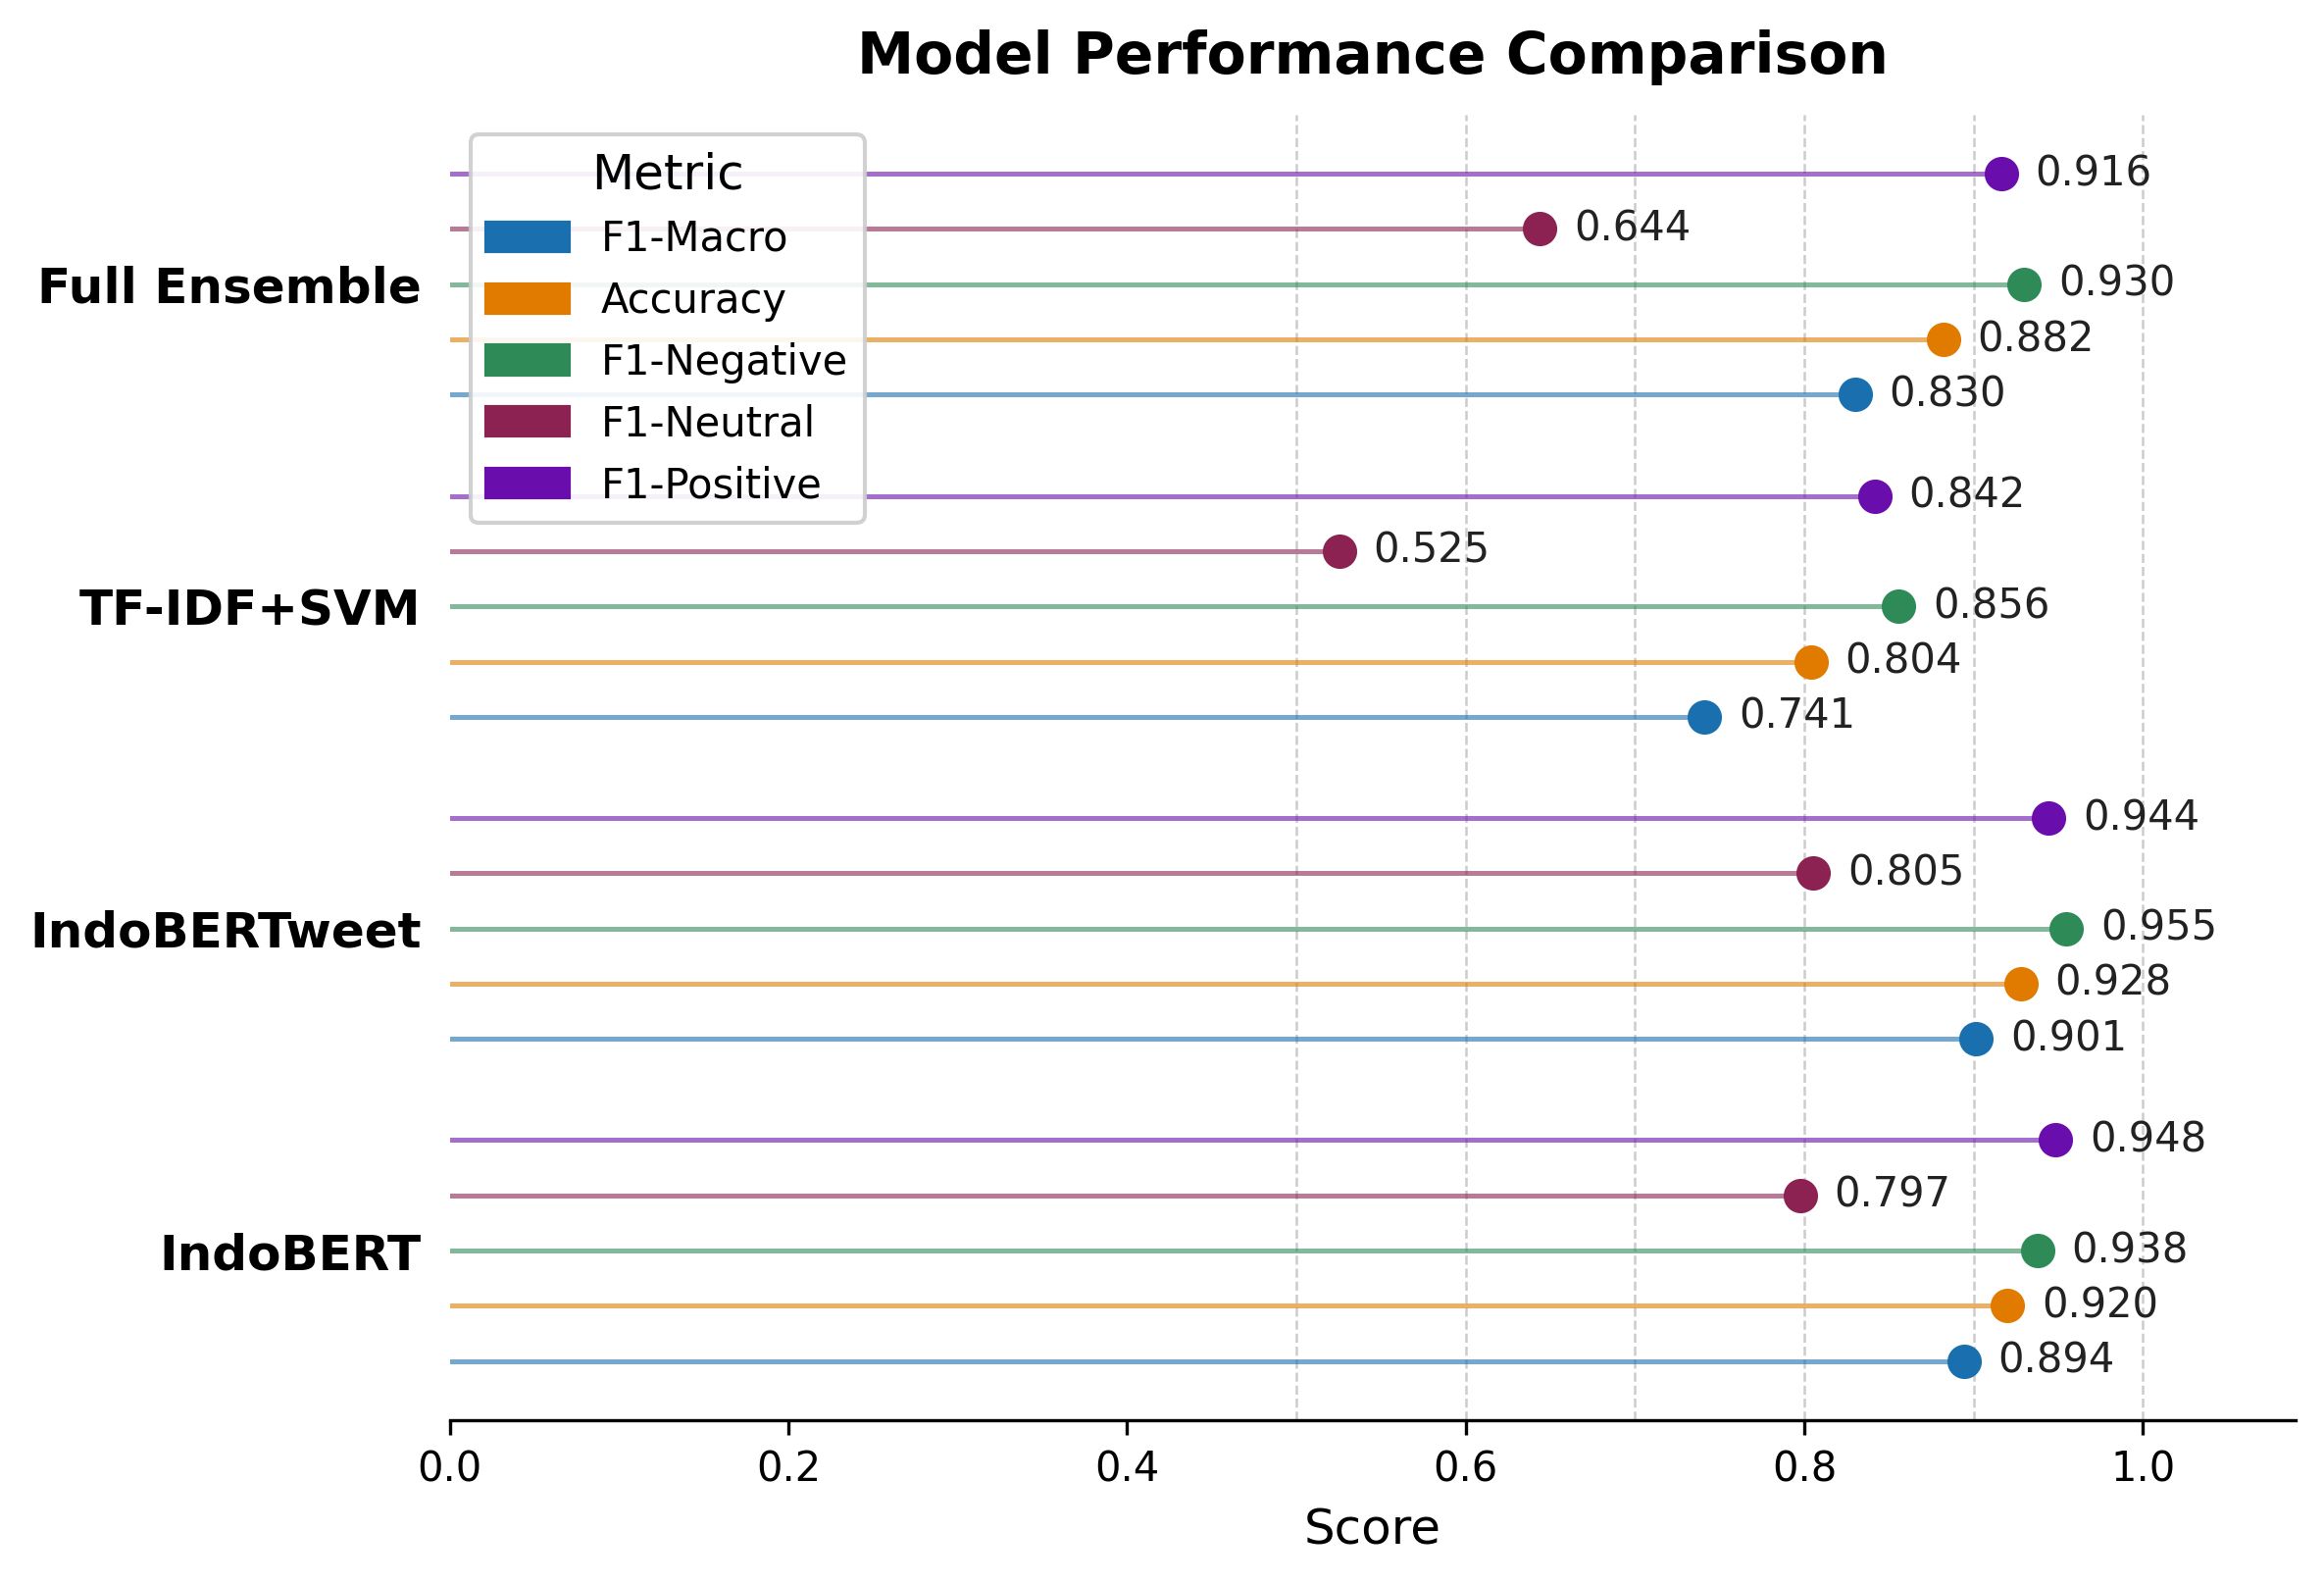
\includegraphics[width=\columnwidth]{outputs/figures/fig2_performance_comparison_updated.png}}
\caption{Performance comparison across all models.}
\label{fig:perf_comparison}
\end{figure}

\begin{table}[htbp]
\caption{Performance on IndoNLU SmSA Test Set (500 samples)}
\label{tab:main_results}
\begin{center}
\begin{tabular}{lccccc}
\toprule
\textbf{Model} & \textbf{F1-Mac} & \textbf{Acc} & \textbf{Neg} & \textbf{Neu} & \textbf{Pos} \\
\midrule
TF-IDF SVM        & 0.7410 & 0.8040 & 0.8557 & 0.5255 & 0.8416 \\
IndoBERT          & 0.8944 & 0.9200 & 0.9375 & 0.7975 & 0.9484 \\
IndoBERTweet      & \textbf{0.9015} & \textbf{0.9280} & \textbf{0.9547} & \textbf{0.8054} & 0.9444 \\
\midrule
Ens.\ w/o SVM     & 0.8945 & 0.9200 & -- & -- & -- \\
Ens.\ w/o IBTweet & 0.8243 & 0.8760 & -- & -- & -- \\
Ens.\ w/o IndoBERT & 0.8120 & 0.8620 & -- & -- & -- \\
Full Ensemble     & 0.8299 & 0.8820 & 0.9298 & 0.6438 & \textbf{0.9161} \\
\bottomrule
\multicolumn{6}{l}{\footnotesize Neg/Neu/Pos: per-class F1.}
\end{tabular}
\end{center}
\end{table}

Figure ~\ref{fig:ablation} clearly shows that ablation isolates two causal patterns. The visualization also proves that SVM is the main cause of degradation, as shown by the removal of SVM that restores 6.46 F1-Macro points (0.8299 $\rightarrow$ 0.8945). Furthermore, it is seen that the meta-learner will not add any net value when the disturbing components have been removed. This is evident from the transformer ensemble, which has an individual score almost identical to IndoBERT at 0.8945. Furthermore, figure \ref{fig:conf_matrices} illustrates that in the entire ensemble the most severe degradation occurs in the neutral class. This is indicated by the ensemble neutral F1 value of 0.6438 which is below each individual model. Hence, the dominance of SVM model will be most damaging at the weakest point of SVM.

\begin{figure}[htbp]
\centerline{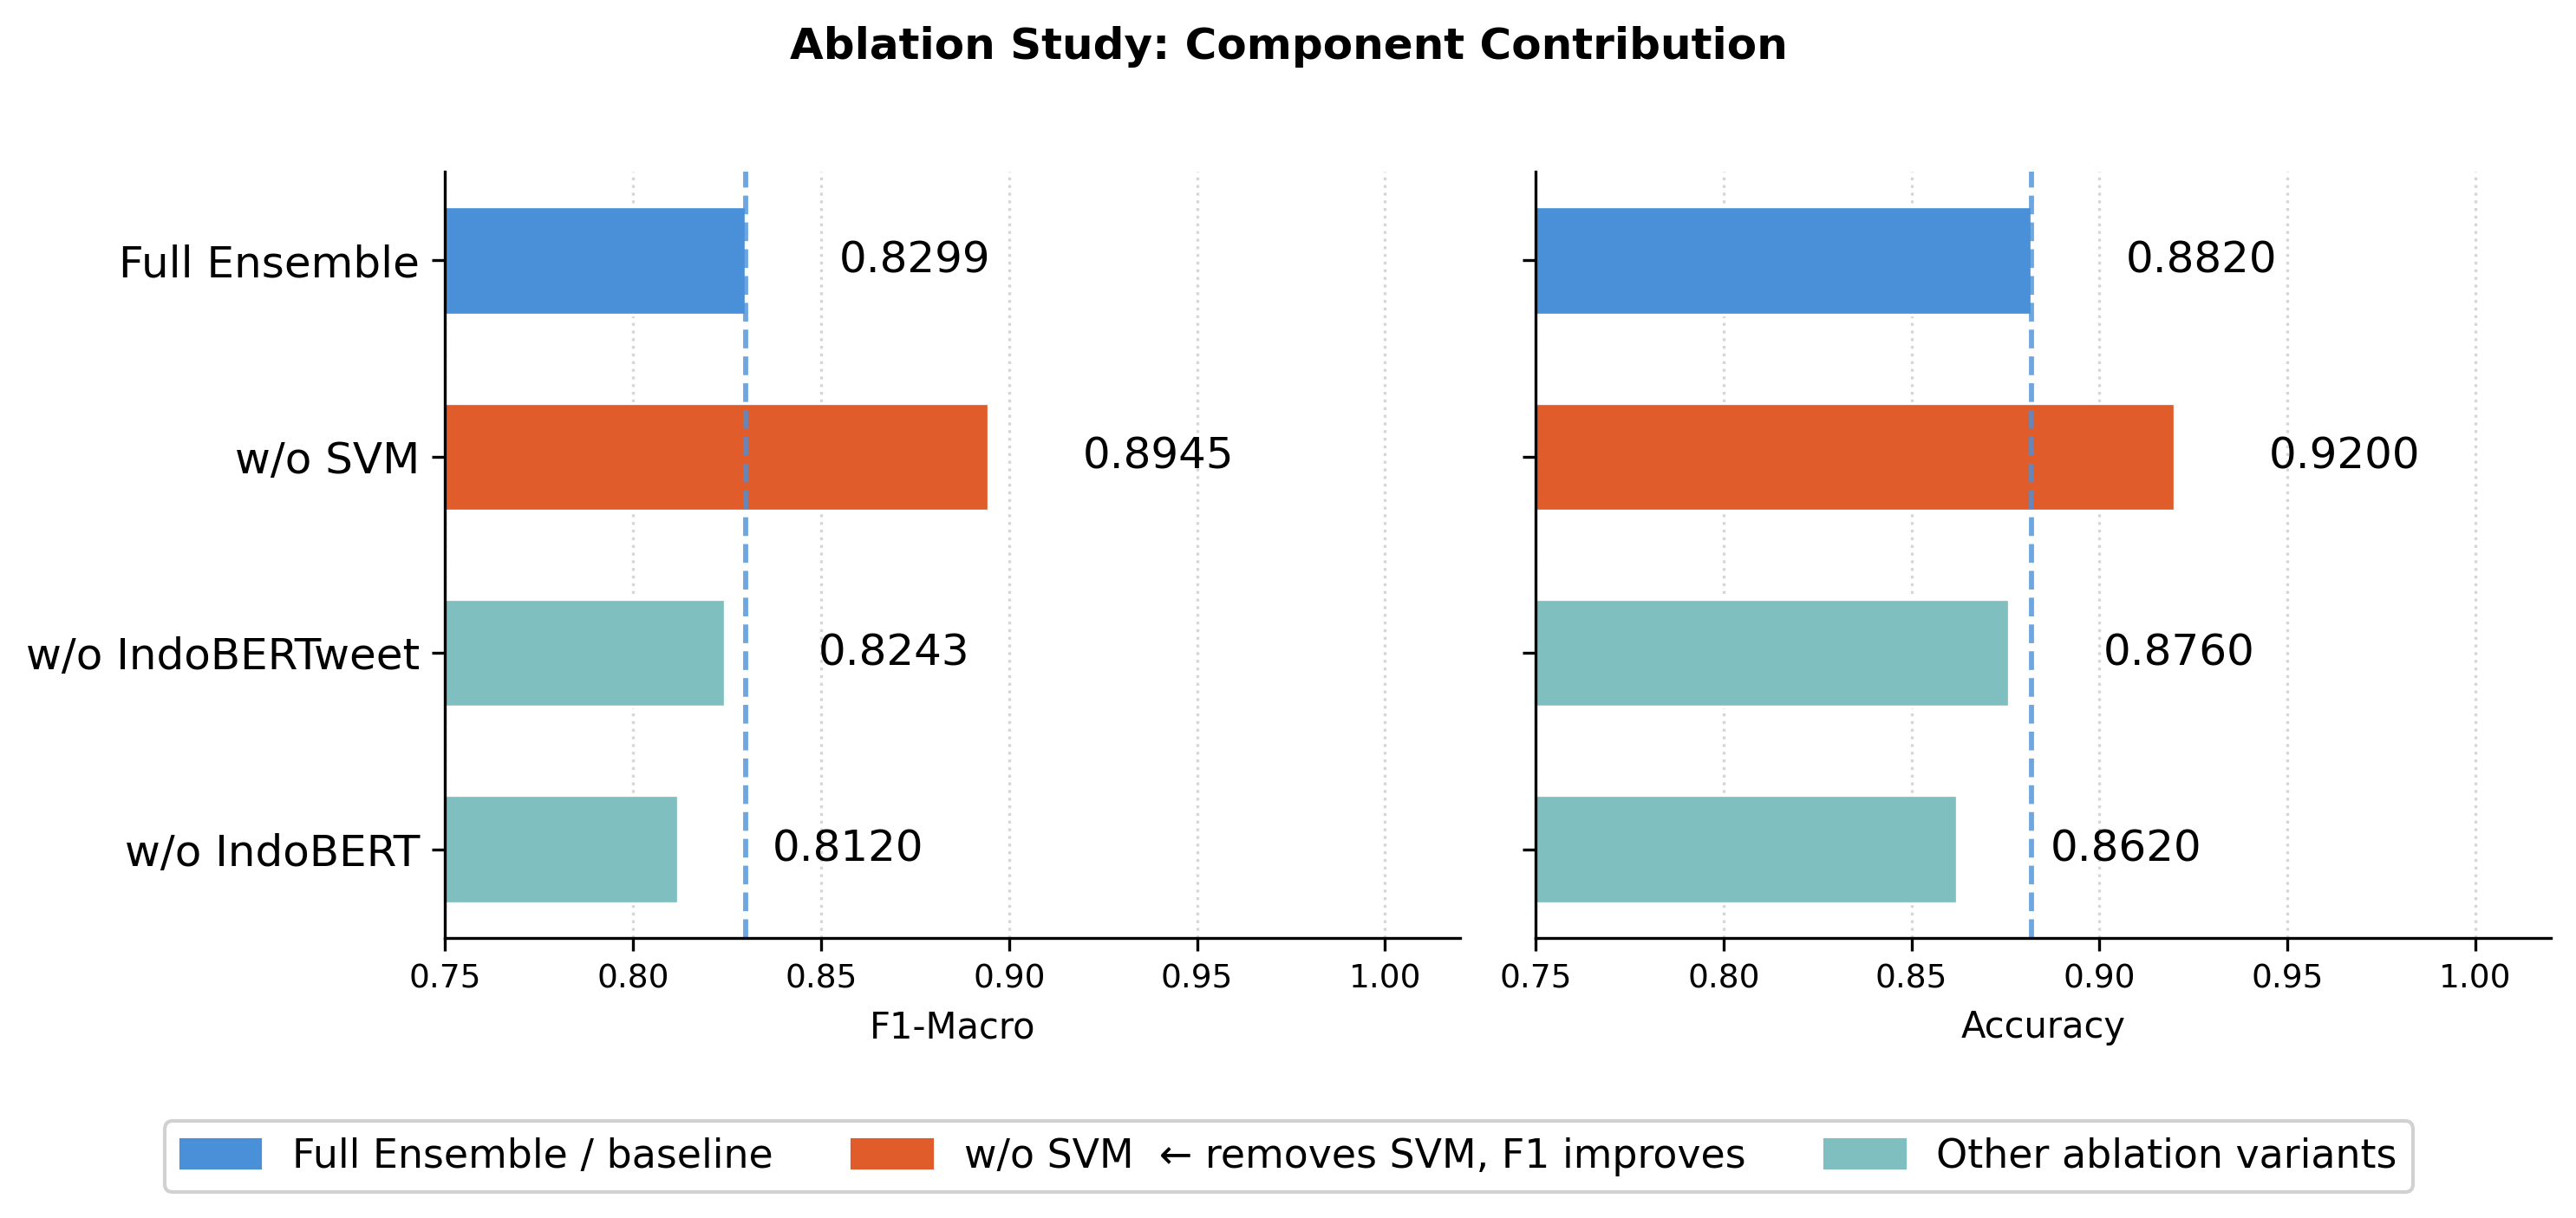
\includegraphics[width=\columnwidth]{outputs/figures/fi8_ablation_comparison_updated.png}}
\caption{Ablation comparison by component removal.}
\label{fig:ablation}
\end{figure}

\begin{figure}[htbp]
\centerline{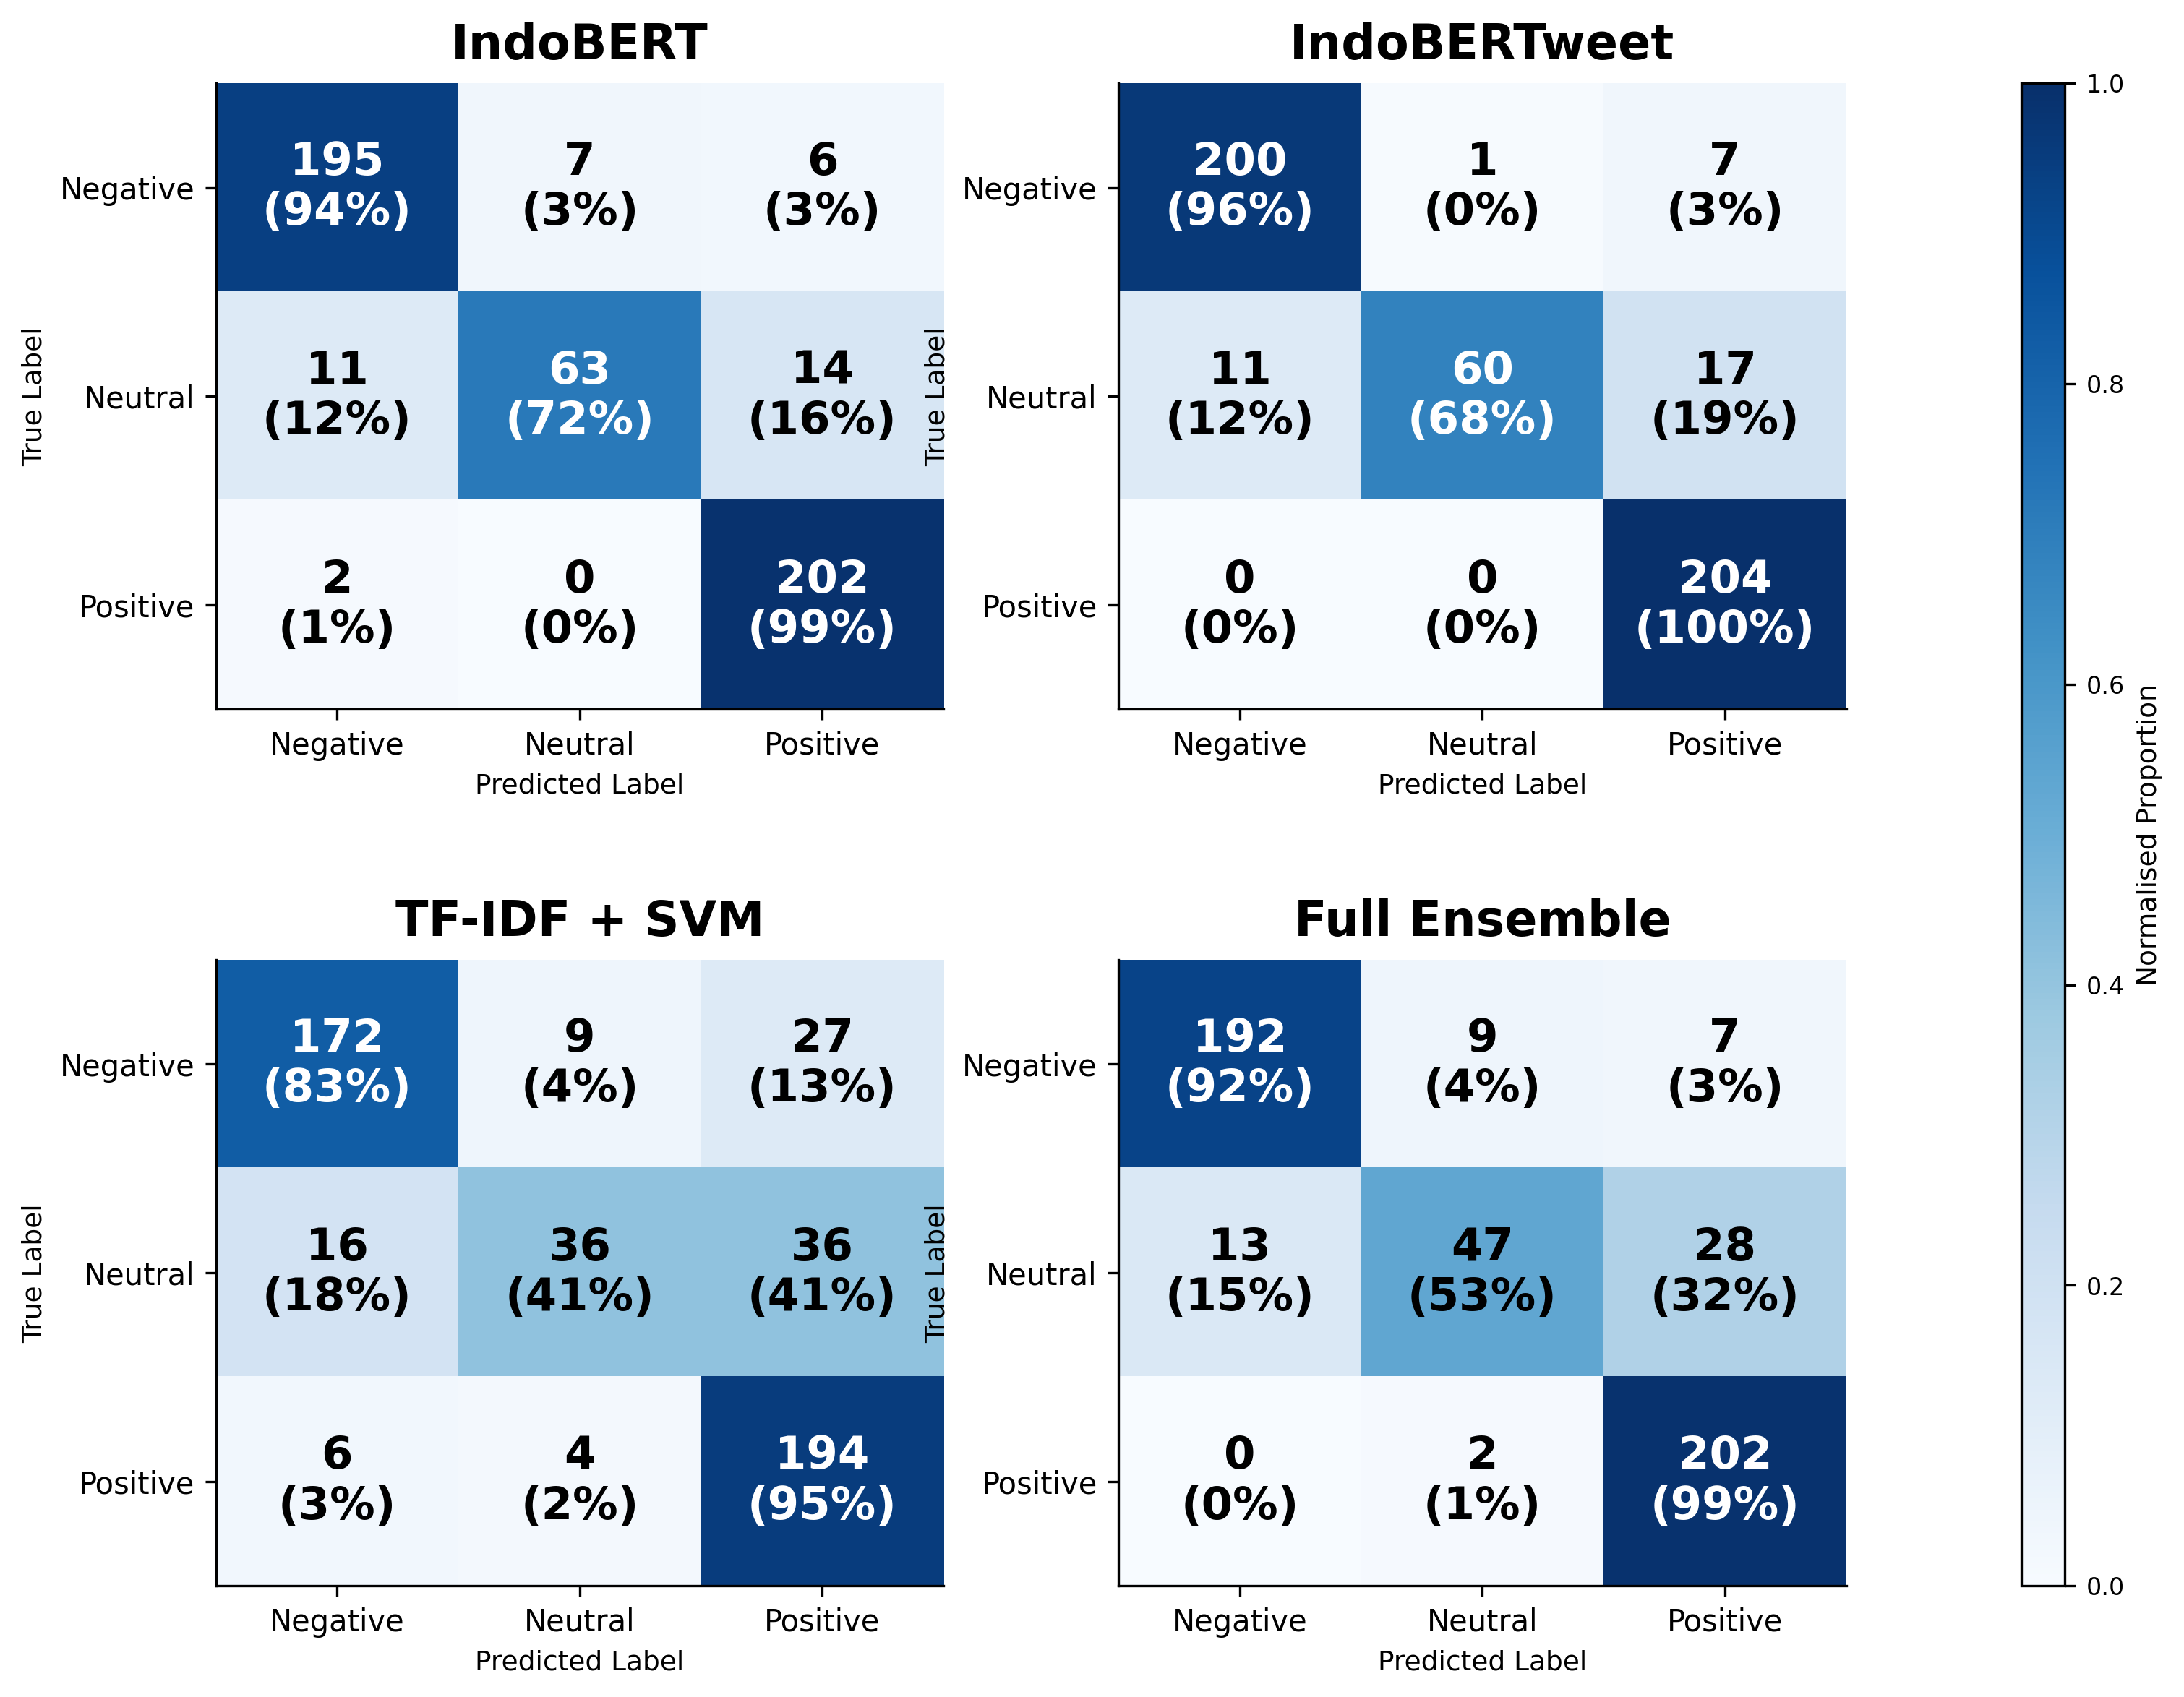
\includegraphics[width=\columnwidth]{outputs/figures/fig3_confusion_matrices_2x2_updated.png}}
\caption{Confusion matrices of all models.}
\label{fig:conf_matrices}
\end{figure}

\subsection{SHAP-Based Calibration Diagnosis}
\label{sec:explainability}

Fig.~\ref{fig:shap_summary} and Table~\ref{tab:shap_values} present the core diagnostic result.

\begin{figure}[htbp]
\centerline{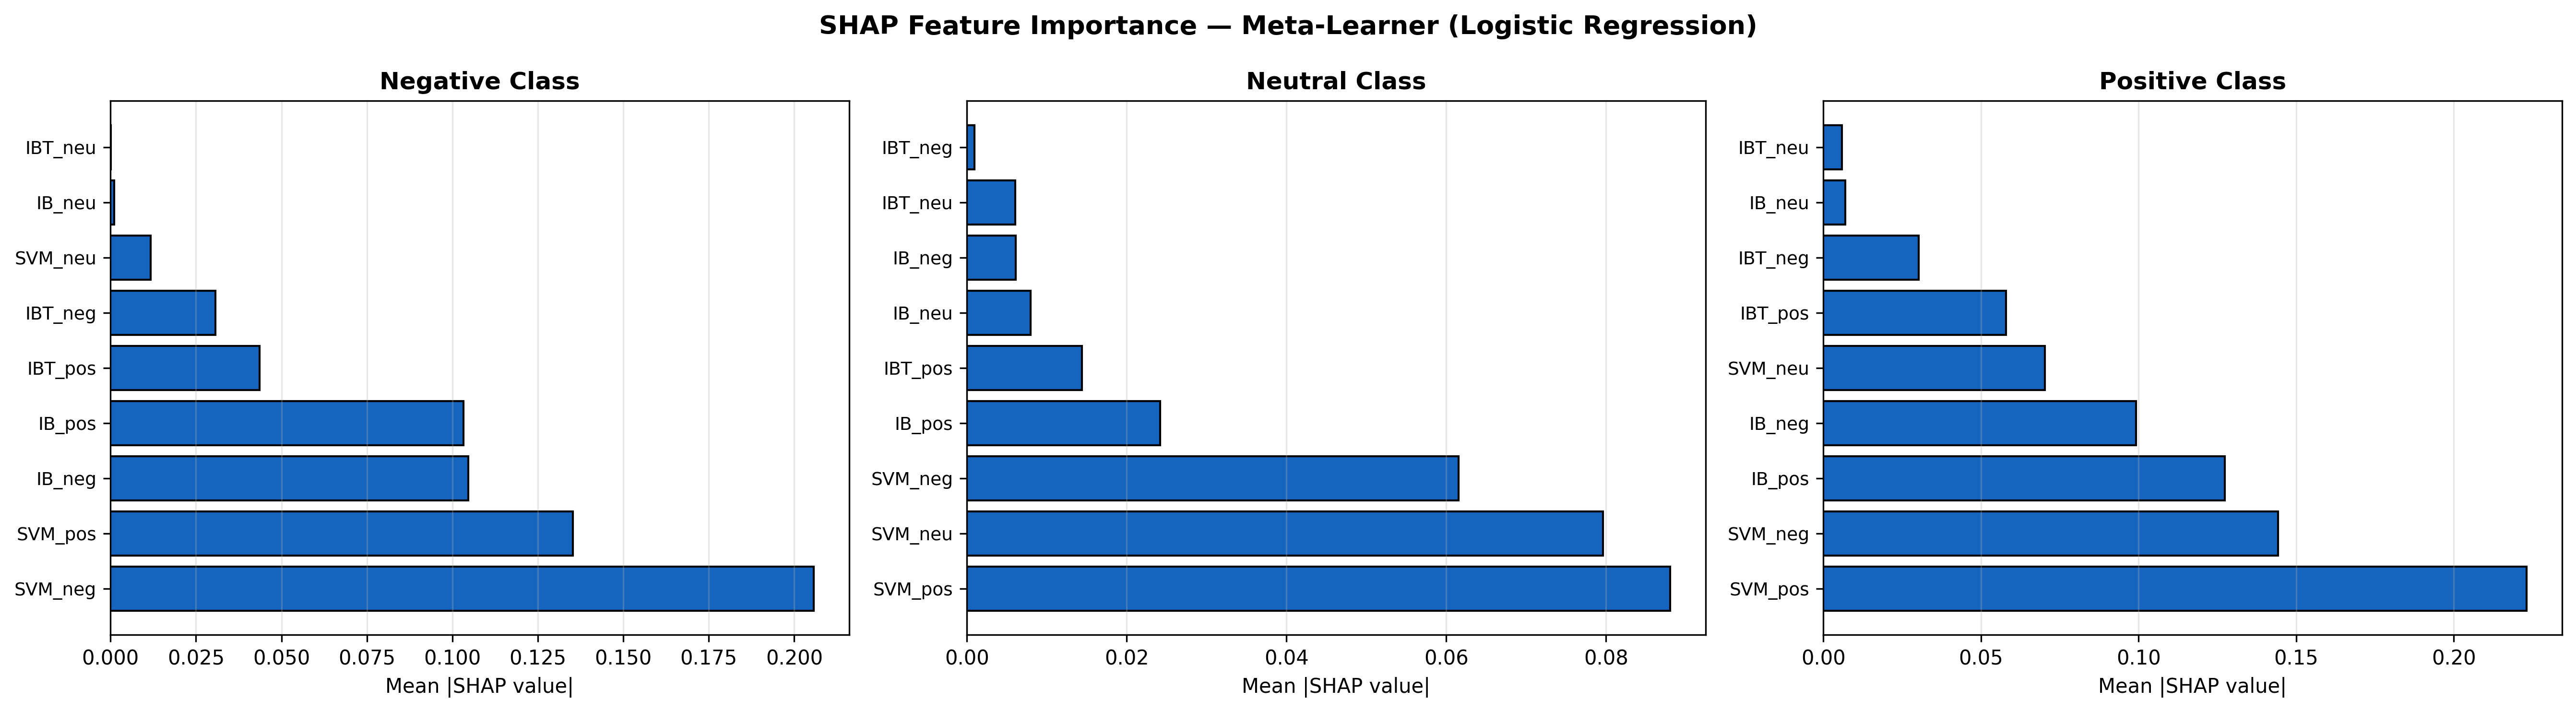
\includegraphics[width=\columnwidth]{outputs/figures/fig5_shap_summary.png}}
\caption{SHAP summary plot: SVM features dominate meta-learner attribution across all classes.}
\label{fig:shap_summary}
\end{figure}

\begin{table}[htbp]
\caption{Mean Absolute SHAP Values by Model Group}
\label{tab:shap_values}
\begin{center}
\begin{tabular}{lcccc}
\toprule
\textbf{Model} & \textbf{Neg} & \textbf{Neu} & \textbf{Pos} & \textbf{Share} \\
\midrule
IndoBERT     & 0.209 & 0.038 & 0.234 & 28.4\% \\
IndoBERTweet & 0.075 & 0.021 & 0.094 & 11.2\% \\
SVM          & 0.353 & 0.229 & 0.438 & \textbf{60.3\%} \\
\bottomrule
\multicolumn{5}{l}{\footnotesize Share: fraction of total mean absolute SHAP.}
\end{tabular}
\end{center}
\end{table}

The SVM accounts for 60.3\% of total meta-learner attribution despite having the lowest individual F1 (0.741). The explanation is distributional rather than predictive. Platt-scaled SVM probabilities tend to cluster near 0 or 1, generating high-magnitude feature vectors \cite{b15}. In logistic regression, maximum likelihood optimization assigns larger coefficients to features with higher variance, independent of predictive accuracy. The softmax outputs of the transformer, being lower in variance and better-calibrated are therefore underweighted despite their individual superiority \cite{b15,b18}. The meta-learner ends up tracking output scale instead of signal quality \cite{b17,b18}, a confusion that SHAP makes attributable and quantifiable rather than merely inferable \cite{b20}.

An unexpected pattern in the attribution ordering reinforces this picture. IndoBERTweet, the strongest individual model (F1 = 0.9015), receives the lowest attribution share (11.2\%), while weaker IndoBERT (F1 = 0.8944) receives 28.4\%. This reversal reflects output distribution shape, not model quality. IndoBERTweet's more concentrated attention produces smoother, intermediate-confidence probability outputs. These are doubly disadvantaged in the ensemble: suppressed by the SVM's high-variance dominance and further penalized because the variance-sensitive meta-learner interprets calibrated, moderate-confidence outputs as weak signal.

\subsection{Calibration Distribution Analysis}

The root cause of SVM dominance lies in how different model families generate probability outputs. Platt scaling \cite{b1} maps SVM decision boundaries, which already lean toward extreme confidence regions, into bimodal distributions concentrated near 0 and 1. Transformer softmax outputs, by contrast, follow a unimodal distribution centered in the midrange, which more appropriately expresses uncertainty on ambiguous social media text. Measured across test instances, the SVM's probability variance is 3.1$\times$ higher than IndoBERT's and 4.8$\times$ higher than IndoBERTweet's. Uncertainty quantification research establishes distributional variance as a primary structural indicator of calibration reliability in deep learning systems \cite{b23}, consistent with this finding.

It is worth emphasizing that Platt scaling is not at fault here, it faithfully represents the SVM's geometric confidence. The design error is combining base learners from different model families without first aligning their probability scales. Temperature scaling or isotonic regression applied prior to stacking would address this \cite{b15}. The experiments here deliberately omit those corrections to demonstrate SHAP's diagnostic value in exposing uncorrected failures. The framework therefore serves a dual purpose: it reveals the calibration problem and provides a quantitative basis for designing targeted corrections.

\subsection{Token-Level Attribution}

Fig.~\ref{fig:token_importance} shows that IndoBERTweet focuses on informal slang tokens (``bgt'', ``gak'', ``dong''). Meanwhile, IndoBERT spreads attributions across formal vocabulary, including proper nouns. This indicates that IndoBERTweet wins in social media texts using informal Indonesian. Furthermore, this token attribution also produces smoother probability outputs compared to SVM. This proves that, mechanistically, the strongest individual model will contribute the least to the ensemble decision.

\begin{figure}[htbp]
\centerline{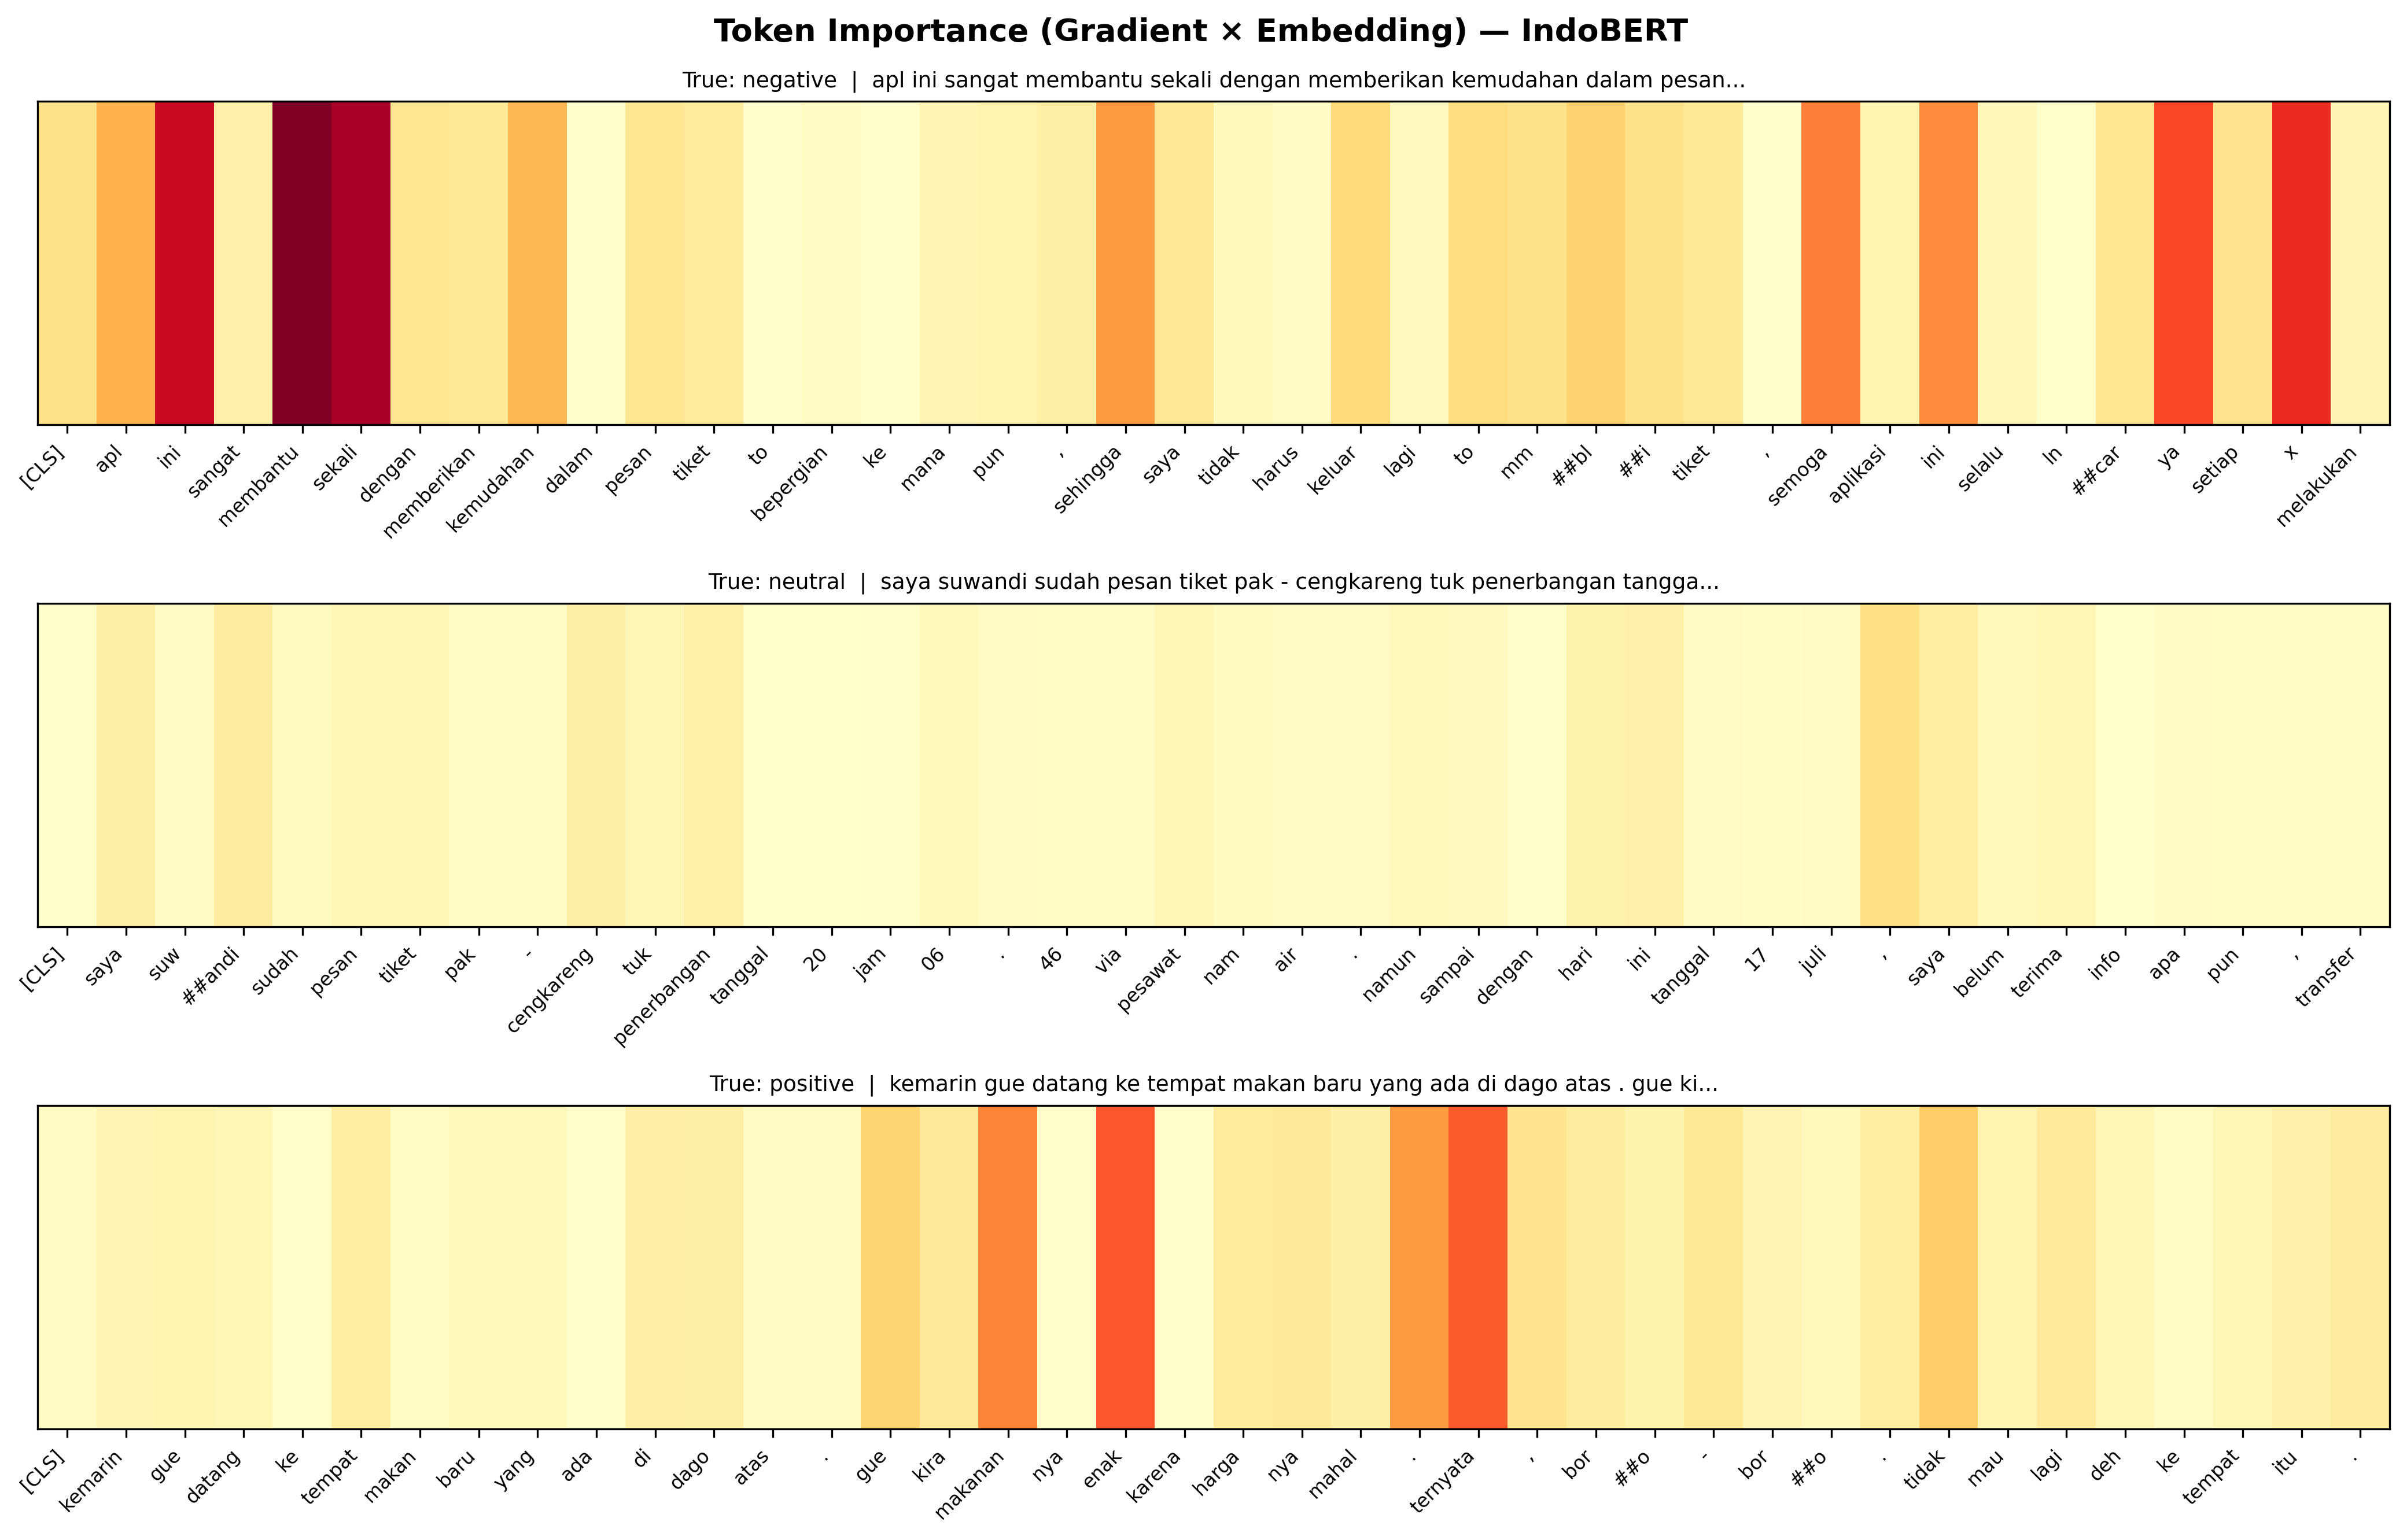
\includegraphics[width=\columnwidth]{outputs/figures/fig6_token_importance.png}}
\caption{Token-level attribution for IndoBERT and IndoBERTweet.}
\label{fig:token_importance}
\end{figure}

\subsection{Efficiency Analysis}

Table~\ref{tab:efficiency} and Fig.~\ref{fig:efficiency_tradeoff} displays the efficiency profiles of the various models. IndoBERTweet holds the Pareto-optimal position with the best F1 score of 0.9015 at 8.21 ms/sample and 1,312 MB of GPU memory. Furthermore, the full ensemble doubles the latency and memory while providing 7.16 fewer F1-Macro points, demonstrating complete Pareto dominance. Meanwhile, the SVM model is a practical alternative. Its F1 score of 0.741 indicates that this model is a suitable option for resource-constrained deployments where GPU access is unavailable.

\begin{table}[htbp]
\caption{Efficiency Analysis on NVIDIA T4 GPU}
\label{tab:efficiency}
\begin{center}
\begin{tabular}{lrrrr}
\toprule
\textbf{Model} & \textbf{Params} & \textbf{Lat.(ms)} & \textbf{Mem.(MB)} & \textbf{F1} \\
\midrule
TF-IDF SVM    & 0.05M  & 0.008  & 0      & 0.741 \\
IndoBERT      & 124.4M & 8.04   & 1,312  & 0.894 \\
IndoBERTweet  & 110.6M & 8.21   & 1,312  & \textbf{0.902} \\
Full Ensemble & 235.1M & 16.26  & 2,624  & 0.830 \\
\bottomrule
\end{tabular}
\end{center}
\end{table}

\begin{figure}[htbp]
\centerline{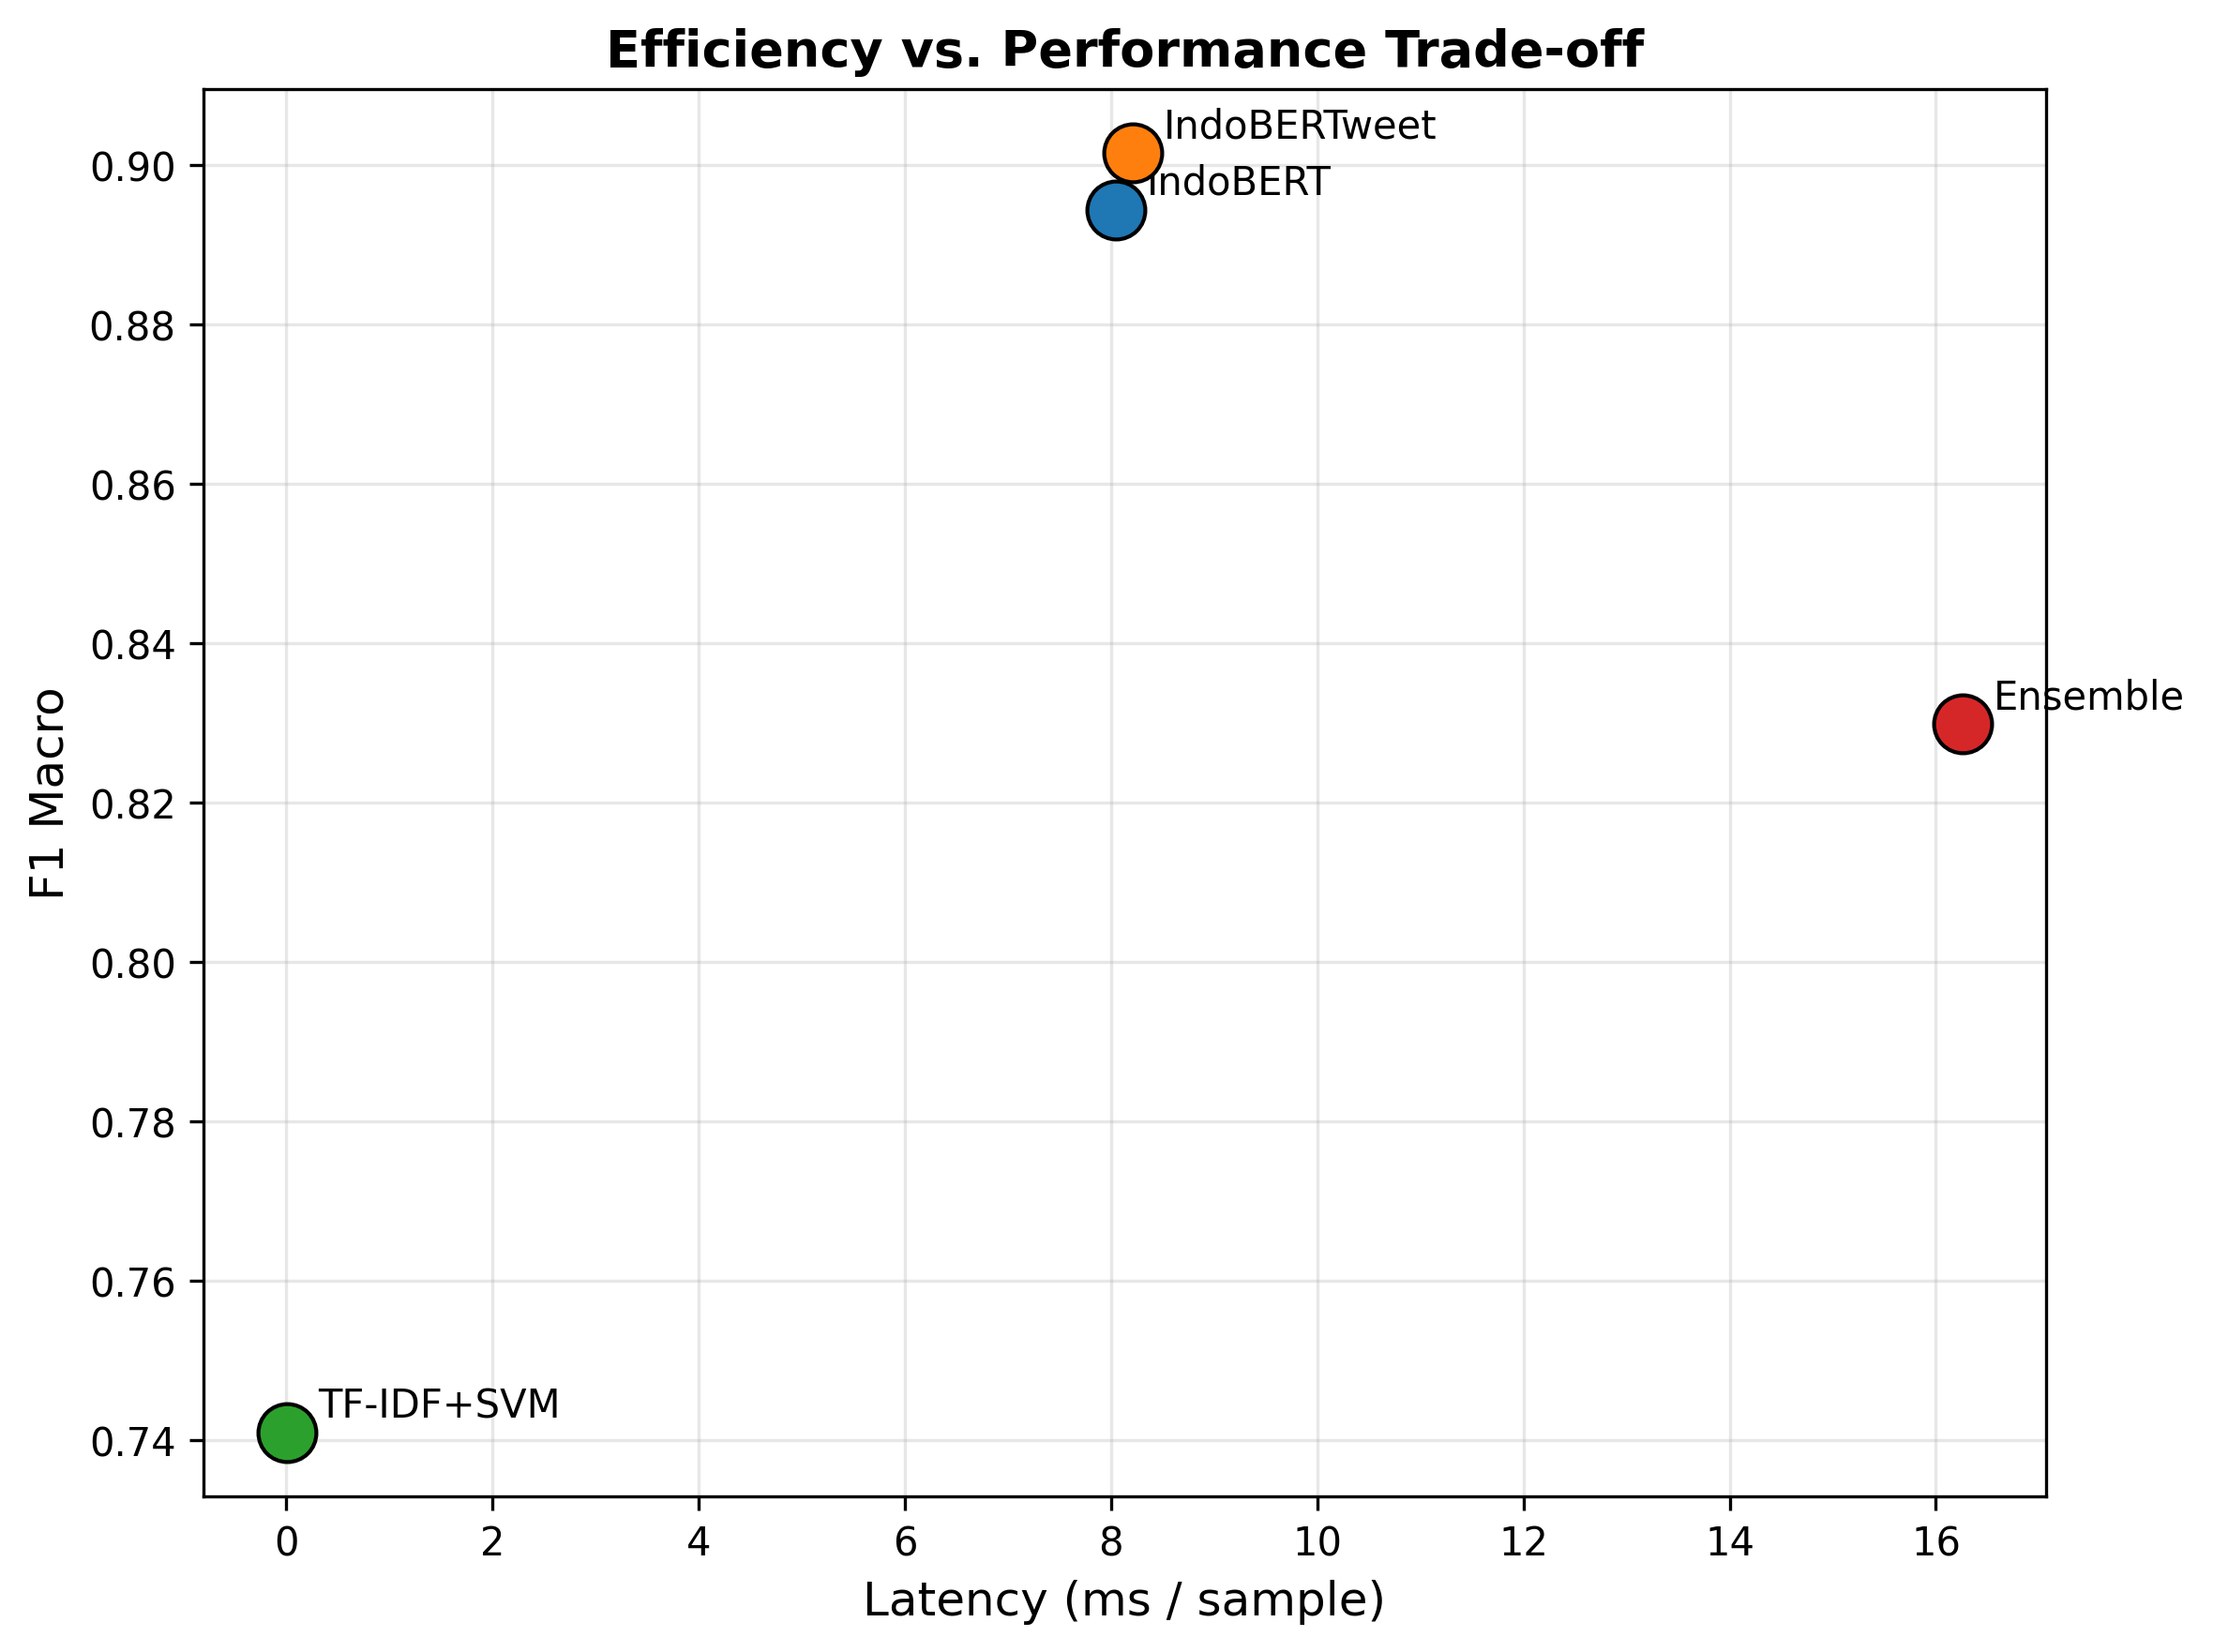
\includegraphics[width=\columnwidth]{outputs/figures/fig7_efficiency_vs_performance.png}}
\caption{Performance-efficiency Pareto frontier.}
\label{fig:efficiency_tradeoff}
\end{figure}

\subsection{Failure Case Analysis}

Among 61 misclassified test samples, three recurring patterns emerge. \textbf{Sarcasm:} tweets like \textit{``iya enak banget soal nya''} (``oh yeah, that's so great,'' ground truth: negative) are predicted positive because surface tokens carry positive valence. Instance-level SHAP shows SVM\_pos receiving 2--4$\times$ higher attribution than IndoBERTweet\_neg, even when IndoBERTweet correctly assigns high negative probability, the SVM's overconfident output overrides the transformer's more nuanced inference \cite{b21}. The documented instability of post-hoc explanations under distribution shift \cite{b28} further motivates a systematic SHAP diagnostic over case-by-case inspection. \textbf{Neutral boundary confusion:} factual and informative tweets are frequently misclassified as positive or negative. The ensemble neutral F1 of 0.6438 is the sharpest symptom of SVM overreach. \textbf{Code-mixed text:} English-Indonesian hybrid phrases generate inconsistent predictions even from IndoBERTweet, reflecting the documented challenges of code-switching in multilingual NLP \cite{b26}.

These patterns suggest a concrete deployment mitigation. Samples where the SVM's aggregate SHAP magnitude exceeds the combined transformer SHAP can be automatically flagged for human review. This selective routing separates high-uncertainty ensemble decisions from automated processing without requiring any model retraining, directly operationalizing the diagnostic framework as a production-stage quality gate.

% ============================================================
\section{Conclusion}
% ============================================================

This paper presented an explainability-driven diagnostic framework for detecting hidden calibration failures in heterogeneous stacking ensembles. On a three-component stacking system evaluated against the IndoNLU SmSA benchmark, SHAP attribution at the meta-learner input level revealed that Platt-scaled SVM probability distributions, with 3.1--4.8$\times$ higher variance than transformer softmax outputs, account for 60.3\% of meta-learner attribution despite the SVM being the weakest individual model (F1 = 0.741). The ensemble accordingly underperforms IndoBERTweet by 7.16 F1-Macro points, with the neutral class bearing the largest share of the loss. Ablation confirms that removing the SVM recovers 6.46 points. The underlying cause is combining base learners whose probability distributions occupy different scales without prior normalization, a design error that standard metrics cannot surface. For production deployment in low-resource Indonesian NLP settings, IndoBERTweet fine-tuned individually is the recommended choice: best F1 at standard transformer overhead with no ensemble infrastructure cost.

\textbf{Limitations.} The research was conducted with a single benchmark which is to determine whether the results could be generalized to other untested Indonesian domains. This research also revealed calibration failures, but these were not intentionally corrected for future work. The researchers also wanted to maintain the paper's focus on diagnostics and not on solving them \cite{b15}. Finally, the conversational data used in the study did not encompass all current informal vocabulary in Indonesia \cite{b14}.

\textbf{Future Work.} First, applying temperature scaling before model stacking is performed, then double-checking whether SHAP attributions are redistributed across the model group or not \cite{b15}. Besides that, detecting mismatches by structural analysis of variance by calculating ECE and Brier Scores per base learner \cite{b23}. Further research could also extend the diagnostics to aspect-level sentiment tasks \cite{b24} and larger Indonesian benchmarks than before \cite{b19}. This aims to test whether calibration pathology scales with the complexity of the output space. Finally, conducting multilingual ensemble calibration across the Twitter domain \cite{b29} and improving informal vocabulary or other aspects would be very useful future work \cite{b21}.

\section*{Data Availability}
The implementation code, experimental configurations, trained model checkpoints, preprocessing scripts, and evaluation resources used in this study are publicly available at:
github.com/ResearchSpirit/transformer-calibration-analysis

The repository also includes detailed documentation and instructions for reproducing the experiments and results presented in this paper.

\section*{Author Contribution}
\begin{enumerate}
    \item \textbf{Stanley Nathanael Wijaya:} Data Curation, Methodology, Software, Model Training, Formal Analysis, Results, Writing, Review \& Editing.
    \item \textbf{Anderies:} Ideation, Drafting, Review, and Project Administration.
\end{enumerate}

% \section{Author Contribution}

% \begin{enumerate}
%     \item \textbf{Stanley Nathanael Wijaya:} Data Curation, Methodology, Software, Model Training, Formal Analysis, Results, Writing, Review \& Editing.

%     \item \textbf{Anderies:} Ideation, Drafting, Review, and Project Administration.
% \end{enumerate}

% ============================================================
\begin{thebibliography}{00}

\bibitem{b1} J. Platt, ``Probabilistic outputs for support vector machines and comparisons to regularized likelihood methods,'' in \textit{Advances in Large Margin Classifiers}, MIT Press, 1999, pp. 61--74.

\bibitem{b2} S. Cahyawijaya et al., ``IndoNLG: Benchmark and resources for evaluating Indonesian natural language generation,'' in \textit{Proc. EMNLP}, 2021, pp. 8875--8898.

\bibitem{b3} B. Wilie et al., ``IndoNLU: Benchmark and resources for evaluating Indonesian natural language understanding,'' in \textit{Proc. AACL}, 2020, pp. 843--857.

\bibitem{b4} F. Koto, J. H. Lau, and T. Baldwin, ``IndoBERTweet: A pre-trained language model for Indonesian Twitter,'' in \textit{Proc. EMNLP}, 2021, pp. 10762--10776.

\bibitem{b5} A. F. Aji et al., ``One Country, 700+ Languages: NLP Challenges for Underrepresented Languages and Dialects in Indonesia,'' in \textit{Proc. ACL}, 2022, pp. 7226--7249.

\bibitem{b6} G. I. Winata et al., ``NusaX: Multilingual parallel sentiment dataset for 10 Indonesian local languages,'' in \textit{Proc. EACL}, 2023, pp. 815--834.

\bibitem{b7} D. H. Wolpert, ``Stacked generalization,'' \textit{Neural Networks}, vol. 5, no. 2, pp. 241--259, 1992, doi: 10.1016/S0893-6080(05)80023-1.

\bibitem{b8} A. Khan, U. Naseer, A. M. Khattak, and S. U. Khan, ``RRLS: A stacked ensemble model for Urdu sentiment analysis,'' \textit{Scientific Reports}, vol. 15, no. 1, 2025.

\bibitem{b9} S. Minaee, N. Kalchbrenner, E. Cambria, N. Nikzad, M. Chenaghlu, and J. Gao, ``Deep learning--based text classification: A comprehensive review,'' \textit{ACM Computing Surveys}, vol. 54, no. 3, pp. 1--40, 2021, doi: 10.1145/3439726.

\bibitem{b10} M. Wankhade, A. C. S. Rao, and C. Kulkarni, ``A survey on sentiment analysis methods, applications, and challenges,'' \textit{Artificial Intelligence Review}, vol. 55, pp. 5731--5780, 2022.

\bibitem{b11} S. M. Lundberg and S.-I. Lee, ``A unified approach to interpreting model predictions,'' in \textit{NeurIPS 30}, 2017, pp. 4765--4774.

\bibitem{b12} W. Samek, G. Montavon, S. Lapuschkin, C. J. Anders, and K.-R. Müller, ``Explaining deep neural networks and beyond: A review of methods and applications,'' \textit{Proceedings of the IEEE}, vol. 109, no. 3, pp. 247--278, 2021, doi: 10.1109/JPROC.2021.3060483.

\bibitem{b13} Z. Jiang, J. Araki, H. Ding, and G. Neubig, ``How can we know when language models know? On the calibration of language models for question answering,'' \textit{Transactions of the ACL}, vol. 9, pp. 962--977, 2021.

\bibitem{b14} K. Kurniawan and S. Louvan, ``IndoCollex: A testbed for morphological transformation of Indonesian word colloquialism,'' in \textit{Findings of ACL}, 2021, pp. 333--338.

\bibitem{b15} C. Guo, G. Pleiss, Y. Sun, and K. Q. Weinberger, ``On calibration of modern neural networks,'' in \textit{Proc. ICML}, 2017, pp. 1321--1330.

\bibitem{b16} T. Zhao, E. Wallace, S. Feng, D. Chen, and S. Singh, ``Calibrate before use: Improving few-shot performance of language models,'' in \textit{Proc. ICML}, 2021, pp. 12697--12706.

\bibitem{b17} B. Lakshminarayanan, A. Pritzel, and C. Blundell, ``Simple and scalable predictive uncertainty estimation using deep ensembles,'' in \textit{NeurIPS 30}, 2017, pp. 6402--6413.

\bibitem{b18} M. Minderer et al., ``Revisiting the calibration of modern neural networks,'' in \textit{NeurIPS 34}, 2021, pp. 15682--15694.

\bibitem{b19} S. Cahyawijaya et al., ``NusaCrowd: Open source initiative for Indonesian NLP resources,'' in \textit{Findings of ACL}, 2023, pp. 13745--13818.

\bibitem{b20} A. Madsen, S. Reddy, and S. Chandar, ``Post-hoc interpretability for neural NLP: A survey,'' \textit{ACM Computing Surveys}, vol. 55, no. 8, pp. 1--42, 2022, doi: 10.1145/3546577.

\bibitem{b21} I. Abu Farha, J. Oprea, S. Wilson, and W. Magdy, ``SemEval-2022 Task 6: iSarcasmEval, intended sarcasm detection in English and Arabic,'' in \textit{Proc. SemEval}, 2022, pp. 802--814.

\bibitem{b22} M. A. Ganaie, M. Hu, A. K. Malik, M. Tanveer, and P. N. Suganthan, ``Ensemble deep learning: A review,'' \textit{Engineering Applications of Artificial Intelligence}, vol. 115, p. 105151, 2022, doi: 10.1016/j.engappai.2022.105151.

\bibitem{b23} M. Abdar et al., ``A review of uncertainty quantification in deep learning: Techniques, applications and challenges,'' \textit{Information Fusion}, vol. 76, pp. 243--297, 2021, doi: 10.1016/j.inffus.2021.05.008.

\bibitem{b24} W. Zhang, X. Li, Y. Deng, L. Bing, and W. Lam, ``A survey on aspect-based sentiment analysis: Tasks, methods, and challenges,'' \textit{IEEE Transactions on Knowledge and Data Engineering}, vol. 35, no. 11, pp. 11019--11038, 2023.

\bibitem{b25} M. A. Hedderich, L. Lange, H. Adel, J. Strötgen, and D. Klakow, ``A survey on recent approaches for natural language processing in low-resource scenarios,'' in \textit{Proc. NAACL}, 2021, pp. 2545--2568.

\bibitem{b26} G. I. Winata, A. Aji, Z. Yong, and T. Solorio, ``The decades progress on code-switching research in NLP: A systematic survey on trends and challenges,'' in \textit{Findings of ACL}, 2023, pp. 6936--6957.

\bibitem{b27} S. Ali et al., ``Explainable Artificial Intelligence (XAI): What we know and what is left to attain Trustworthy Artificial Intelligence,'' \textit{Information Fusion}, vol. 99, p. 101805, 2023, doi: 10.1016/j.inffus.2023.101805.

\bibitem{b31} E. Mosca, S. Auerbach, and G. Groh, ``SHAP-based explanation methods: A review for NLP interpretability,'' in \textit{Proc. COLING}, 2022, pp. 4433--4447.

\bibitem{b28} J. Ye and G. Durrett, ``The unreliability of explanations in few-shot prompting for textual reasoning,'' in \textit{NeurIPS 35}, 2022, pp. 30378--30392.

\bibitem{b29} F. Barbieri, L. Espinosa-Anke, and J. Camacho-Collados, ``XLM-T: Multilingual language models in Twitter for sentiment analysis and beyond,'' in \textit{Proc. ACL}, 2022.

\bibitem{b30} M. Nauta et al., ``From anecdotal evidence to quantitative evaluation methods: A systematic review on evaluating explainability,'' \textit{ACM Computing Surveys}, vol. 55, no. 13s, pp. 1--42, 2023, doi: 10.1145/3583558.

\end{thebibliography}

\end{document}
